Verification is the process of ensuring the governing equations are correctly solved in FESTIM.
This is an integral part of every simulation code for it guarantees the code is error free.
It is generally hard to simply substitute this process by code comparison (cross-checks between two different codes) because often the codes are implemented differently.
Moreover, if the code we are comparing with is not verified, then obtaining similar results does not give any guarantee on the code accuracy as two different codes can have the same bug.

Several methods can be used to verify a code but the Method of Exact Solutions (MES) and the Method of Manufactured Solutions (MMS) are employed here.

Both methods consist in comparing a computed solution with an exact solution and measuring the error.
The exact solution in the MES is obtained by solving the governing equations analytically.
When using the MMS, the problem is reversed: an arbitrary exact solution (called \textit{manufactured solution}) is chosen and injected in the governing equations.
It is then possible to determine source terms and boundary conditions.
These are then fed into the code and the computed solution is compared to the manufactured (exact) solution.

This MMS is often used to unravel the complexity of governing equations \sidecite{dudson_verification_2016, roache_code_2002}.
This is particularly useful when dealing with complex geometries or to exercise non-trivial material propoerties.

This section describes two verification cases of FESTIM.
The first one uses the MES and the second one the MMS.
More complex and thorough verification cases are shown in Appendix \ref{appendix verification}.

\subsubsection{Case 1: H transport (MES)} \label{analytical}

\begin{figure}
    \centering
    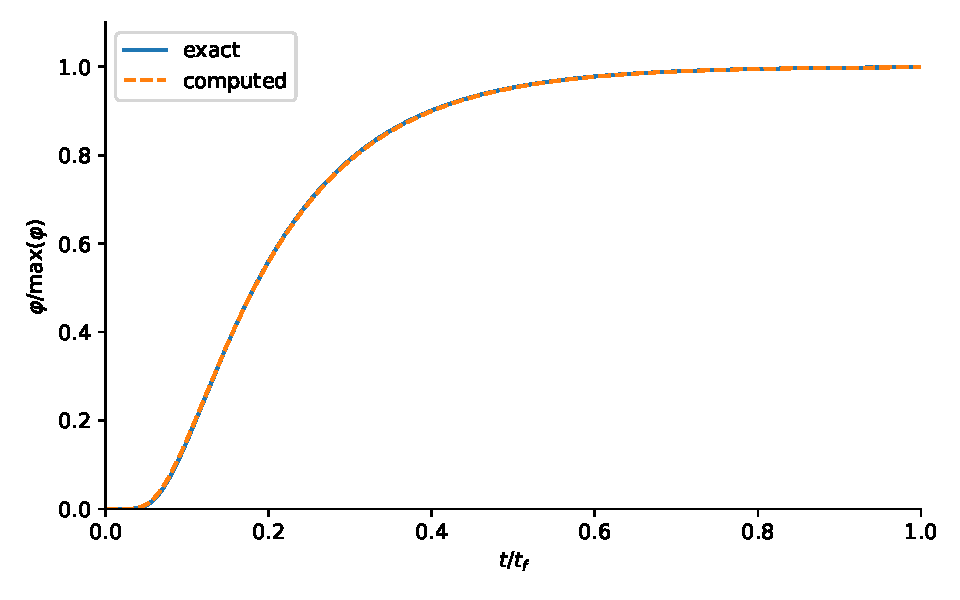
\includegraphics[width=\linewidth]{Figures/Chapter3/mes_festim_effective_diffusion.pdf}
    \caption{Temporal evolution of the outward particle flux $\varphi$ at $x=l$ (Case 1).}
    \label{fig:FESTIM vs analytical}
\end{figure}

% Although validation against experiments could show that FESTIM is able reproduce the data with a given set of parameters, objective verification against analytical solutions is first required to ensure that the governing Equations \ref{eq:mobile} and \ref{eq:trapped} are solved correctly.

For this verification case, a 1D slab is considered with a thickness $l$.
The concentration of mobile particles was set to $c_0$ on one side of the slab and set to zero on the other side.
Only one trap is considered in this case and its density $n$ is homogeneously distributed.

The trapping parameter $\zeta$ is defined in \sidecite{longhurst_verification_2005} as follow:
\begin{equation}
    \zeta = \frac{p}{k \: n} + \frac{c_\mathrm{m}}{n}
\end{equation}

In our case, we choose the trapping and detrapping rates $k$ and $p$, the concentration $c_0$ and the temperature $T$ so that $\zeta \gg \frac{c_\mathrm{m}}{n}$.
This is known as the \textit{effective diffusivity regime} where the diffusion is almost identical to the case where there are no traps.
In this regime, the governing equations are identical as a pure diffusion regime and are therefore easy to solve analytically.

The coefficient $D$ is then replaced by an effective diffusion coefficient:
\begin{equation}
    D_\mathrm{eff} = \frac{D}{1+\frac{1}{\zeta}}
\end{equation}
The particle flux at the background surface ($x=l$) is expressed in $\si{H.m^{-2}.s^{-1}}$ and finally defined in \sidecite{longhurst_verification_2005} by:
\begin{equation}
    \varphi(t) = \frac{c_0 D}{l}\bigg[1+2\sum_{m=1}^{\infty}(-1)^m \exp\bigg(-m^2\frac{\pi^2 \:D_\mathrm{eff} \: t}{l^2}\bigg)\bigg]
\label{eq:flux analytical}
\end{equation}
Note: The infinite sum has been truncated at $m=10000$.

All the parameters are defined in Table \ref{tab:parameters analytical verification}.
These parameters have been chosen for the sake of verification and do not necessarily represent realistic conditions as verification is a mathematical exercise.
\begin{table}
    \centering
    \begin{tabular}{p{2.3cm} p{2cm} r}
        Parameter & Units & Value \\
        \hline
        \\
        $D_0$ & $\si{m^2.s^{-1}}$ & 2.0 \\
        $k_0$ & $\si{m^3.s^{-1}}$ & 0.01 \\
        $p_0$ & $\si{s^{-1}}$ & 1.0 \\
        \\
        $E_D$ & $\si{eV}$ & 0.2 \\
        $E_k$ & $\si{eV}$ & 0.1 \\
        $E_p$ & $\si{eV}$ & 0.1 \\
        \\
        $c_0$ & $\si{m^{-3}}$ & 2.0 \\
        $n$ & $\si{m^{-3}}$ & 2.0 \\
        $l$ & $\si{m}$ & 1.5\\
        \\
        $T$ & $\si{K}$ & 300 \\
        \\
        $t_f$ & $\si{s}$ & 2000 \\
        \\
    \end{tabular}
    \caption{Parameters used for the analytical verification (Case 1).}
    \label{tab:parameters analytical verification}
\end{table}
One can notice on Figure \ref{fig:FESTIM vs analytical} that the numerical results are in good agreement with the analytical solution.
The relative L2 error between analytical and numerical solutions was found to be \approx 1 \% with 1000 piecewise linear elements (P1) and a stepsize of \SI{1}{s}.
This value decreases with the stepsize and with the element size (see \reffig{MES evolution of L2 error as function of dt and dx}).
\begin{figure}
    \centering
    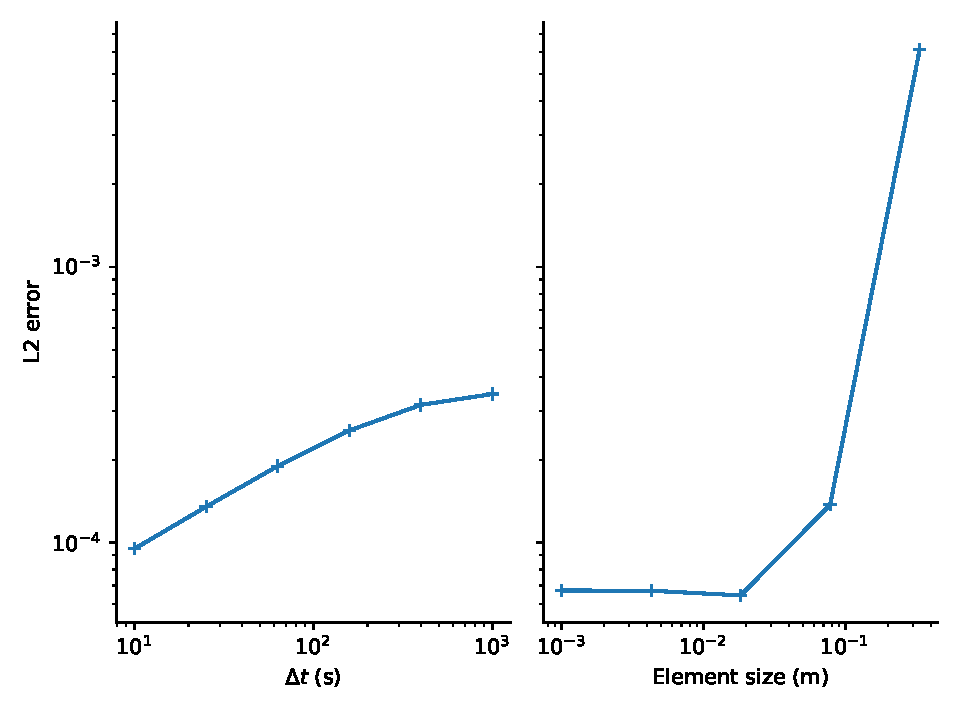
\includegraphics[width=\linewidth]{Figures/Chapter2/error_vs_element_size_and_dt.pdf}
    \caption{Evolution of the L2 error on $\varphi$ as a function of the stepsize and element length (Case 1).}
    \labfig{MES evolution of L2 error as function of dt and dx}
\end{figure}


Since this test case is very similar to a pure diffusion case, it does not exercise all terms of the governing equations.
To do so, the governing equations would have to be solved for a generic case which proves to be complex.
This is why the MMS will be used instead.

\subsubsection{Case 2: H transport (MMS)} \label{mms}

\paragraph{Principle}
The MMS is often used to unravel the complexity of governing equations \sidecite{dudson_verification_2016, roache_code_2002}.
This is particularly useful when dealing with complex geometries or to exercise non-trivial material properties.

The principle of the MMS is to manufacture an exact solution.
Again, physical realism is not a concern here as verification is a mathematical exercise.
This manufactured solution needs to be non trivial in order to test the robustness of the implementation.
It is then passed through the governing equations (either the heat equation or the hydrogen transport equations) and source terms are obtained.

Let us take a simple example with the Poisson equation defined on a 1D domain $[x_1, x_2]$:
\begin{equation}
    \frac{\partial u}{\partial t} = \frac{\partial^2 u}{\partial x^2} + q
    \labeq{poisson eq demo mms}
\end{equation}
where $u$ is the unknown, $q$ is the source term.

The manufactured solution is arbitrarily defined as:
\begin{equation}
    U(t, x) = A + \sin{(x + B t)}
\end{equation}
where $A$ and $B$ are real numbers, $t$ is the time, and $x$ is the spatial coordinate.
By replacing $u$ by $U(t, x)$ in \refeq{poisson eq demo mms}, we can identify the source term $q$ that would produce the solution $U(t, x)$:

\begin{equation}
    Q(t, x) = B \cos{(x + B t)} + \sin{(x + B t)}
\end{equation}

Several boundary conditions can be used to produce $U(t, x)$.
We can for instance set a Dirichlet boundary condition on the boundaries $x=x_1$ and $x=x_2$:
\begin{align}
    u(t, x_1) &= U(t, x_1) \\
    u(t, x_2) &= U(t, x_2)
\end{align}

or Neumann boundary conditions:
\begin{align}
    \frac{\partial u(t, x)}{\partial x}\Big | _{ x=x_1} &= \frac{\partial U(t, x)}{\partial x} \Big | _{ x=x_1} \\
    \frac{\partial u(t, x)}{\partial x}\Big | _{ x=x_2} &= \frac{\partial U(t, x)}{\partial x} \Big | _{ x=x_2}
\end{align}

or even a combination of Dirichlet and Neumann boundary conditions.

By solving \refeq{poisson eq demo mms} with $q = Q(t, x)$ and initial condition $u = U(0, x)$, we can obtain the computed solution $u_\mathrm{computed}$.
The error between the computed solution $u_\mathrm{computed}$ and the exact solution $U(t, x)$ can be calculated to assess the 

\paragraph{Case 2a: Application to 1D hydrogen transport}

Let us apply the MMS to the hydrogen transport model on a 1D domain $\Omega$.
In order to exercise all terms in Equations \ref{eq:mobile} and \ref{eq:trapped}, the following manufactured solutions are chosen:
\begin{equation}
    \begin{cases}
    c_{m_D} = 1 + x^2 + \sin(t) \\
    c_{{t,1}_D} = 1 + x^2 + \cos(t)
    \end{cases}
    \label{eq: manufactured solutions}
\end{equation}

By combining Equations \ref{eq:mobile}, \ref{eq:trapped} and \ref{eq: manufactured solutions}, one can obtain the following source terms:
\begin{equation}
    \begin{cases}
    f = \cos(t) - \sin(t) - 2D \\
    g_1 = \nu_1 c_{{t,1}_D} - \nu_m c_{m_D} ( n_1 - c_{{t,1}_D}) - \sin(t)
    \end{cases}
    \label{eq:sources}
\end{equation}
$f$ is the source term of the mobile concentration equation and $g_1$ is the source term of the trapped concentration equation.

where $g_1$ is an additional source term in Equation \ref{eq:trapped}.
The Dirichlet boundary conditions for $c_\mathrm{m}$ and $c_{t,1}$ are:

\begin{equation}
    \begin{cases}
    c_\mathrm{m} = 1 + x^2 + \sin(t) \quad \text{on } \partial \Omega \\
    c_{t,1} = 1 + x^2 + \cos(t) \quad \text{on } \partial \Omega 
    \end{cases}
\end{equation}
where $\partial\Omega$ is the boundary of the domain.
Finally, initial values for $c_\mathrm{m}$ and $c_{t,i}$ are:
\begin{equation}
    \begin{cases}
    c_\mathrm{m}(t=0) = 1 + x^2 \\
    c_{t,1}(t=0) = 2 + x^2
    \end{cases}
\end{equation}
Once all these parameters are fed into FESTIM, one can easily compare the computed solution with the exact solution in Equation \ref{eq: manufactured solutions}.
The L2-norm $E_{c_\mathrm{m}}$ can then be calculated as follow:
\begin{equation}
    E_{c_\mathrm{m}} = \sqrt{\int_\Omega(c_{m_D} - c_\mathrm{m})^2dx}
\end{equation}
The evolution of $E_{c_\mathrm{m}}$ as function of the element size $h$ is shown on Figure \ref{fig:error vs h}.
One can notice that $E_{c_\mathrm{m}}$ increases as $A\cdot h^k$.
This is known as the \textit{asymptotic regime} and the coefficient $k$ is called the convergence rate.
$k$ typically approaches $N+1$ as $h$ approaches zero, $N$ being the order of the finite elements.
In this case, $k \approx 2$ as expected since first order finite elements have been used.

\begin{figure}
    \centering
    \includegraphics[width=1\linewidth]{"Figures/Chapter3/L2 error on Cm vs h"}
    \caption{Evolution of the L2 norm of the error as function of element size h for the 1D H transport case (Case 2a).}
    \label{fig:error vs h}
\end{figure}

\paragraph{Case 2b: Application to 2D hydrogen transport}


The same method can be applied to a 2D case.
Let us choose the following steady state test problem on a domain $\Omega = [0, 1] \times [0, 1]$ with the manufactured solution $c_D(x, y) = \sin(\omega \pi x) \sin(\omega \pi y)$.

\begin{align}
    \nabla \cdot D \nabla c_\mathrm{m} &= -f_1 \\
    k c_\mathrm{m} (n - c_\mathrm{t}) - p c_\mathrm{t} &= -f_2 \\
    c_\mathrm{m} &= c_\mathrm{t} = c_D \text{  on  } \partial \Omega \\
    D &= 2 \\
    p &= 3 \\
    k &= 2 \\
\end{align}

The source terms $f_1$ and $f_2$ and the boundary conditions can be obtained in a similar fashion by replacing $c_\mathrm{m}$ and $c_\mathrm{t}$ in the governing equations.

It was shown that the computed solutions was similar to the exact solutions (see Figure \ref{fig: results MMS 2D H transport}).
Moreover, the convergence rates confirm the mesh dependency of the computed solutions accuracy (see Figure \ref{fig: convergence rates H}).
% A super-convergence is observed for the P2 elements.

\begin{figure*}
    \centering
    \begin{subfigure}{0.3\linewidth}
        \centering
        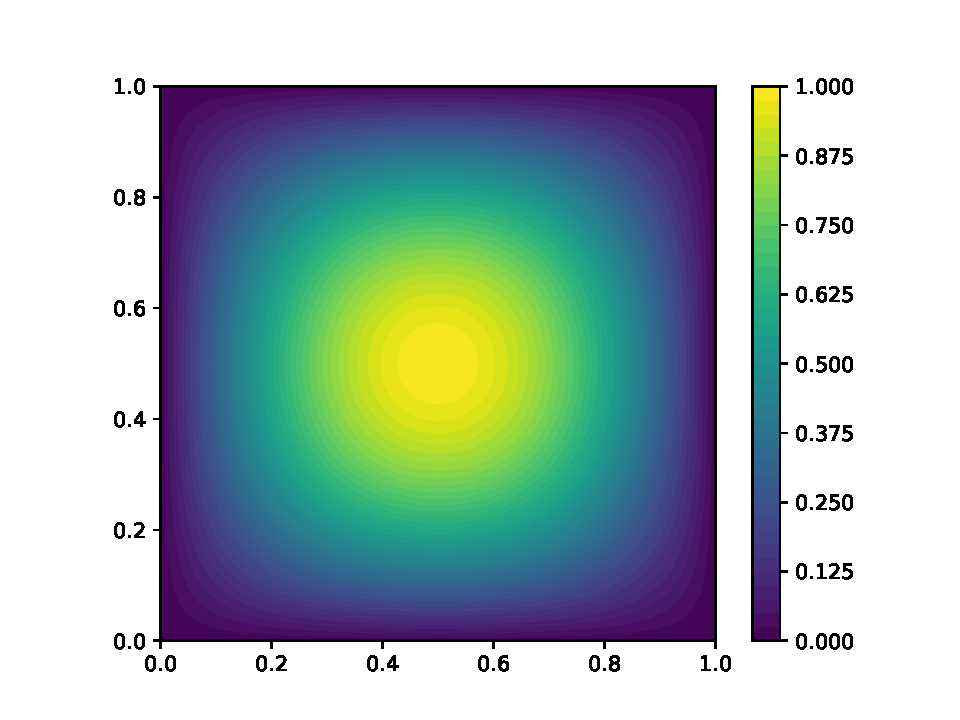
\includegraphics[width=\linewidth]{Figures/Chapter2/c_m.pdf}
        \caption{Computed $c_\mathrm{m}$ (64 elements)}
    \end{subfigure}%
    \begin{subfigure}{0.3\linewidth}
        \centering
        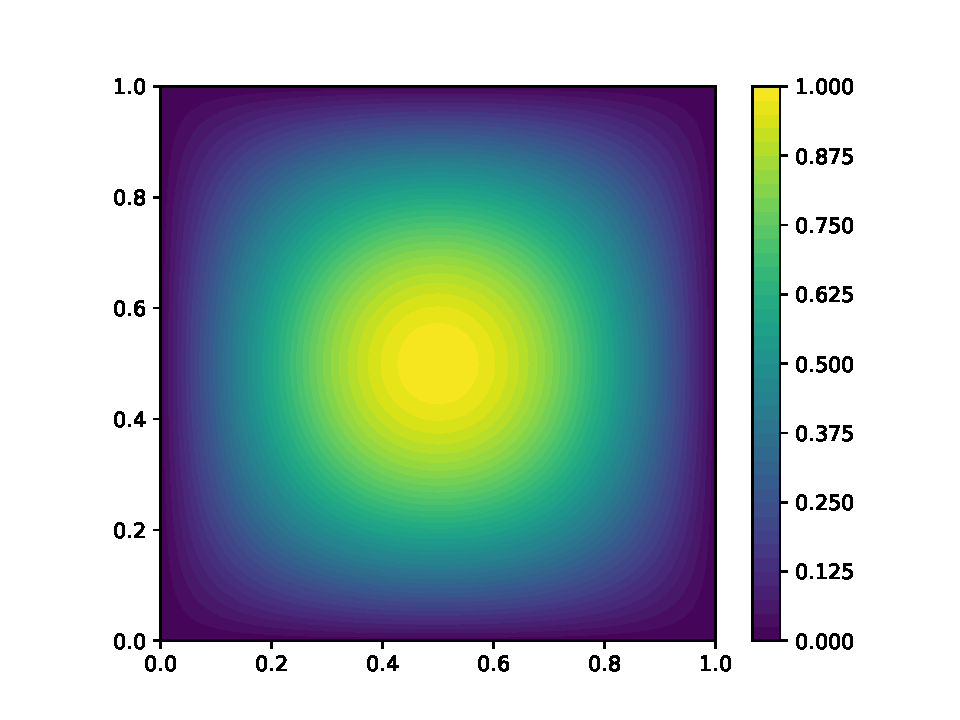
\includegraphics[width=\linewidth]{Figures/Chapter2/c_t.pdf}
        \caption{Computed $c_\mathrm{t}$ (64 elements)}
    \end{subfigure}%
    \begin{subfigure}{0.3\linewidth}
        \centering
        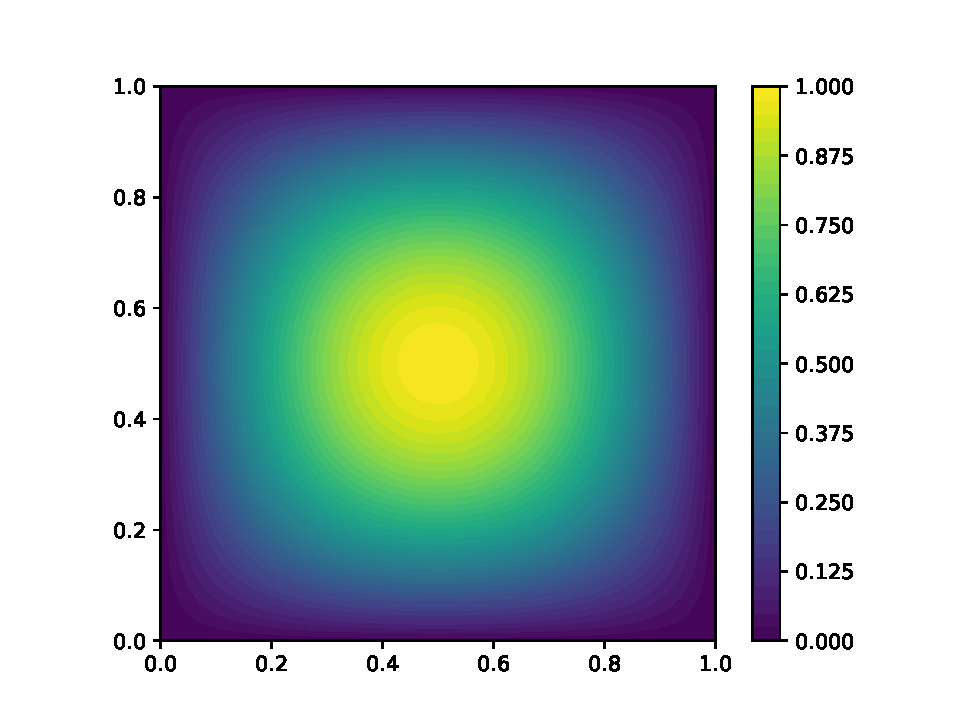
\includegraphics[width=\linewidth]{Figures/Chapter2/c_exact.pdf}
        \caption{Exact solution $c_D$}
    \end{subfigure}
    \caption{Comparison of the computed concentrations with the exact solution (Case 2b).}
    \label{fig: results MMS 2D H transport}
\end{figure*}

\begin{figure}
    \centering
    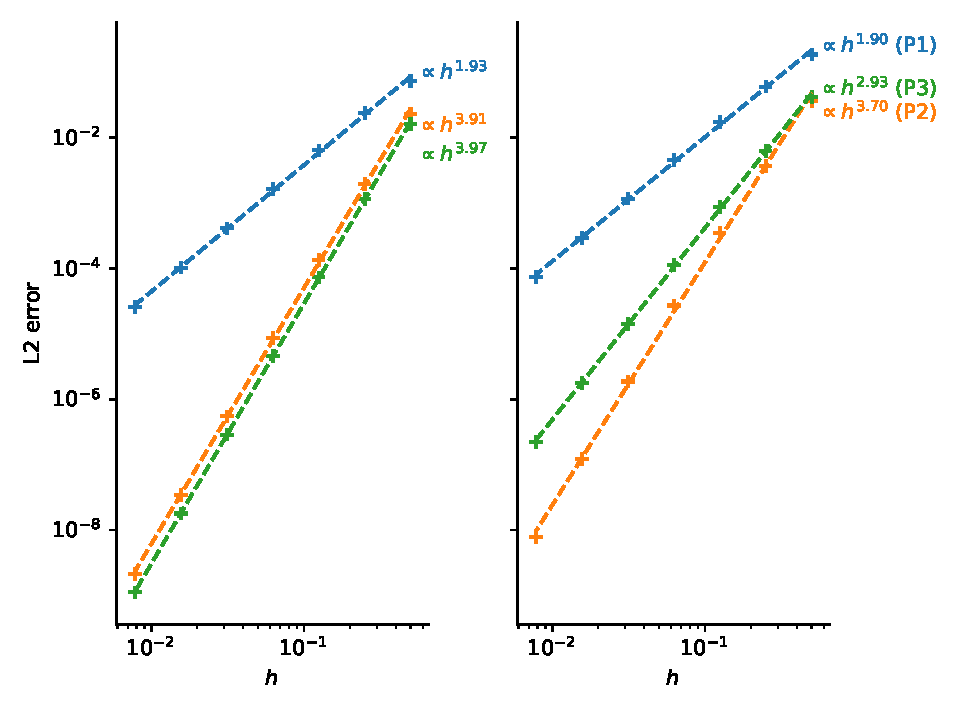
\includegraphics[width=\linewidth]{Figures/Chapter2/convergence_rate_H.pdf}
    \caption{Evolution of the L2 error on $c_\mathrm{m}$ (left) and $c_\mathrm{t}$ (right) showing the convergence rates for the 2D H transport case (Case 2b).}
    \label{fig: convergence rates H}
\end{figure}
